
\section{Introduction}
\iffalse
TODO:
\begin{itemize}
    \item Explicar el problema. Soluciones propuestas hasta ahora. Por qué no son suficientes. En qué consiste la nuestra.
    \item Definición general aplicación propuesta. Validez para PoS card fraud or internet frauds (CNP: Card Not Present frauds)... pero que hemos concretado en el caso de los ATM fraud.
    \fmc{Poner aquí contexto sobre los distintos tipos de fraude y sus estadísticas: referencia al informe SEPA ("Seventh report on card fraud typos")}
    \item Explicar cómo está organizado el documento.
\end{itemize}
\fi

Although from a classical point of view  databases are thought of for persistent data, nowadays this perspective is changing since data are in motion, continuously changing and (possibly) unbounded. So, the following questions arise: (i) What is the proper data model? and (ii) What is the proper query model? 

\noindent
Regarding the data model, the new nature of data requires a \emph{de facto} new database paradigm -\emph{continuously evolving  databases}- where data can be both \emph{stable} and \emph{volatile}. Even though evolving databases can be implemented according to any approach, graph databases seem especially well suited  here \textcolor{blue}{\cite{GDB-angles2008survey, GDB-kumar2015graph}}. Indeed, the natural way to process evolving graphs as streams of edges gives insights on how to proceed in order to maintain dynamic graph databases.  Hence, we consider that a suitable data model is a \emph{continuously evolving data graph}, a graph having persistent (\emph{stable}) as well as non persistent (\emph{volatile}) relations. Stable relations correspond to edges occurring in standard graph databases while volatile relations are edges arriving in data streams during a set time interval. Once this time interval is over, the relations are not longer valid so that there is no need to store them in the (stable) graph database. However,  when required -as for further legal or auditing purposes- timestamped occurrences of volatile relations can  be kept in a log file. Volatile relations induce subgraphs that exist only while the relations are still valid. Without loss of generality, in this work we consider property graphs (PG) \cite{PG-angles2017foundations, angles2018propertyGraphDatabaseModel} as the basic reference data model. As an example, Figure \ref{fig:constinuousPGa} depicts part of a schema of a PG database where stable relations correspond to the data that a bank typically gathers on its issued cards, ATMs (Automated Teller Machines) network, etc. Volatile relations model the interaction between cards and ATM entities. Concerning the query model, fixed queries evaluated over data streams are known as \emph{continuous queries} \cite{CQ-babu2001continuous,CQ-zaniolo2012logical}. Thus, instead of classical query evaluation processes we envision \emph{incremental/progressive} query evaluation processes. 
%
A query on a PG database can be seen as a PG graph pattern with constraints over some of its properties. Evaluating such a query consists on identify if there is a subgraph of the database that matches the given pattern and satisfies its constraints. 
%Thus, we consider a continuous query as a property-constrained graph pattern to be continuously identified in an evolving PG database. 
The problem of progressively identify and enumerate bitriangles (i.e. a specific graph pattern) in bipartite evolving graphs using the \emph{Dynamic Pipeline Approach} \cite{DP-pasarella2024computational} have been successfully solved by Royo-Sales \cite{DP-bitriangles2021}.  We claim that the problem of evaluating continuous queries over \emph{continuously evolving PGs} belongs to the same family of problems and hence, we propose to address it using the same stream processing approach. However, in this case, in addition to identify the query pattern, the constraint satisfaction over properties must be checked also. Figure \ref{fig:constinuousPGb} shows a constrained graph pattern corresponding to a continuous query.
%
In this work, as a proof of concept,  we tackled the problem of evaluating continuous queries corresponding to anomalous patterns of ATM transactions against a continuously evolving PG representing a bank database. To be concrete, the  anomalous patterns of ATM transactions are identified in the volatile (PG) subgraph of the considered database. The evaluation process is based on the dynamic pipeline computational model and  emits  answers (alarms) as soon as anomalous patterns are identified. Additionally, a log of all the volatile relations of the PG is maintained.  Figure \ref{fig:theProblem} illustrates a possible anomalous situation associated to this query.
%
\begin{figure*}[t!]
    \centering
    \begin{subfigure}[b]{0.6\textwidth}
        \centering
        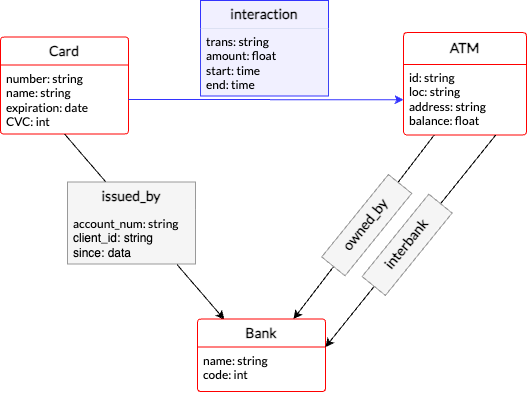
\includegraphics[width=0.55\textwidth]{images/schema.png}
        \caption{Part of a schema of a PG}
         \label{fig:constinuousPGa}
    \end{subfigure}%
     ~ 
    \begin{subfigure}[b]{0.4\textwidth}
        \centering
        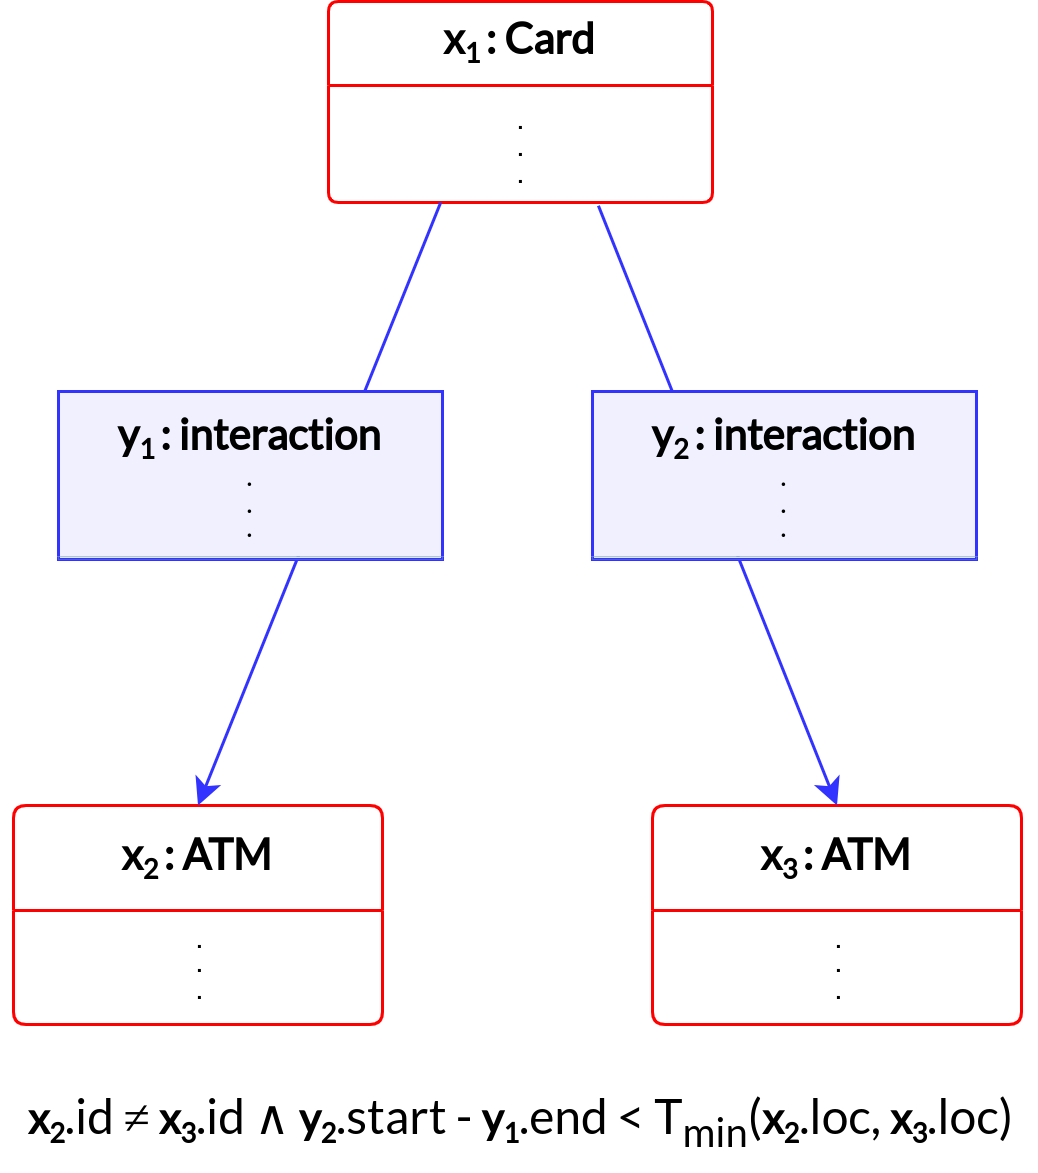
\includegraphics[width=0.55\textwidth]{images/graphPattern.png}
        \caption{Pattern of anomalous transactions}
        \label{fig:constinuousPGb}
    \end{subfigure}
    \caption{Part of a PG schema specifying volatile (\textsf{interaction} edges) and stable  (\textsf{issued\_by, owned\_by, interbank} edges) relations in an evolving ATM Network and a continuous query pattern.}
    \label{fig:constinuousPG}
\end{figure*}
%
\begin{figure}[h]
         \centering
         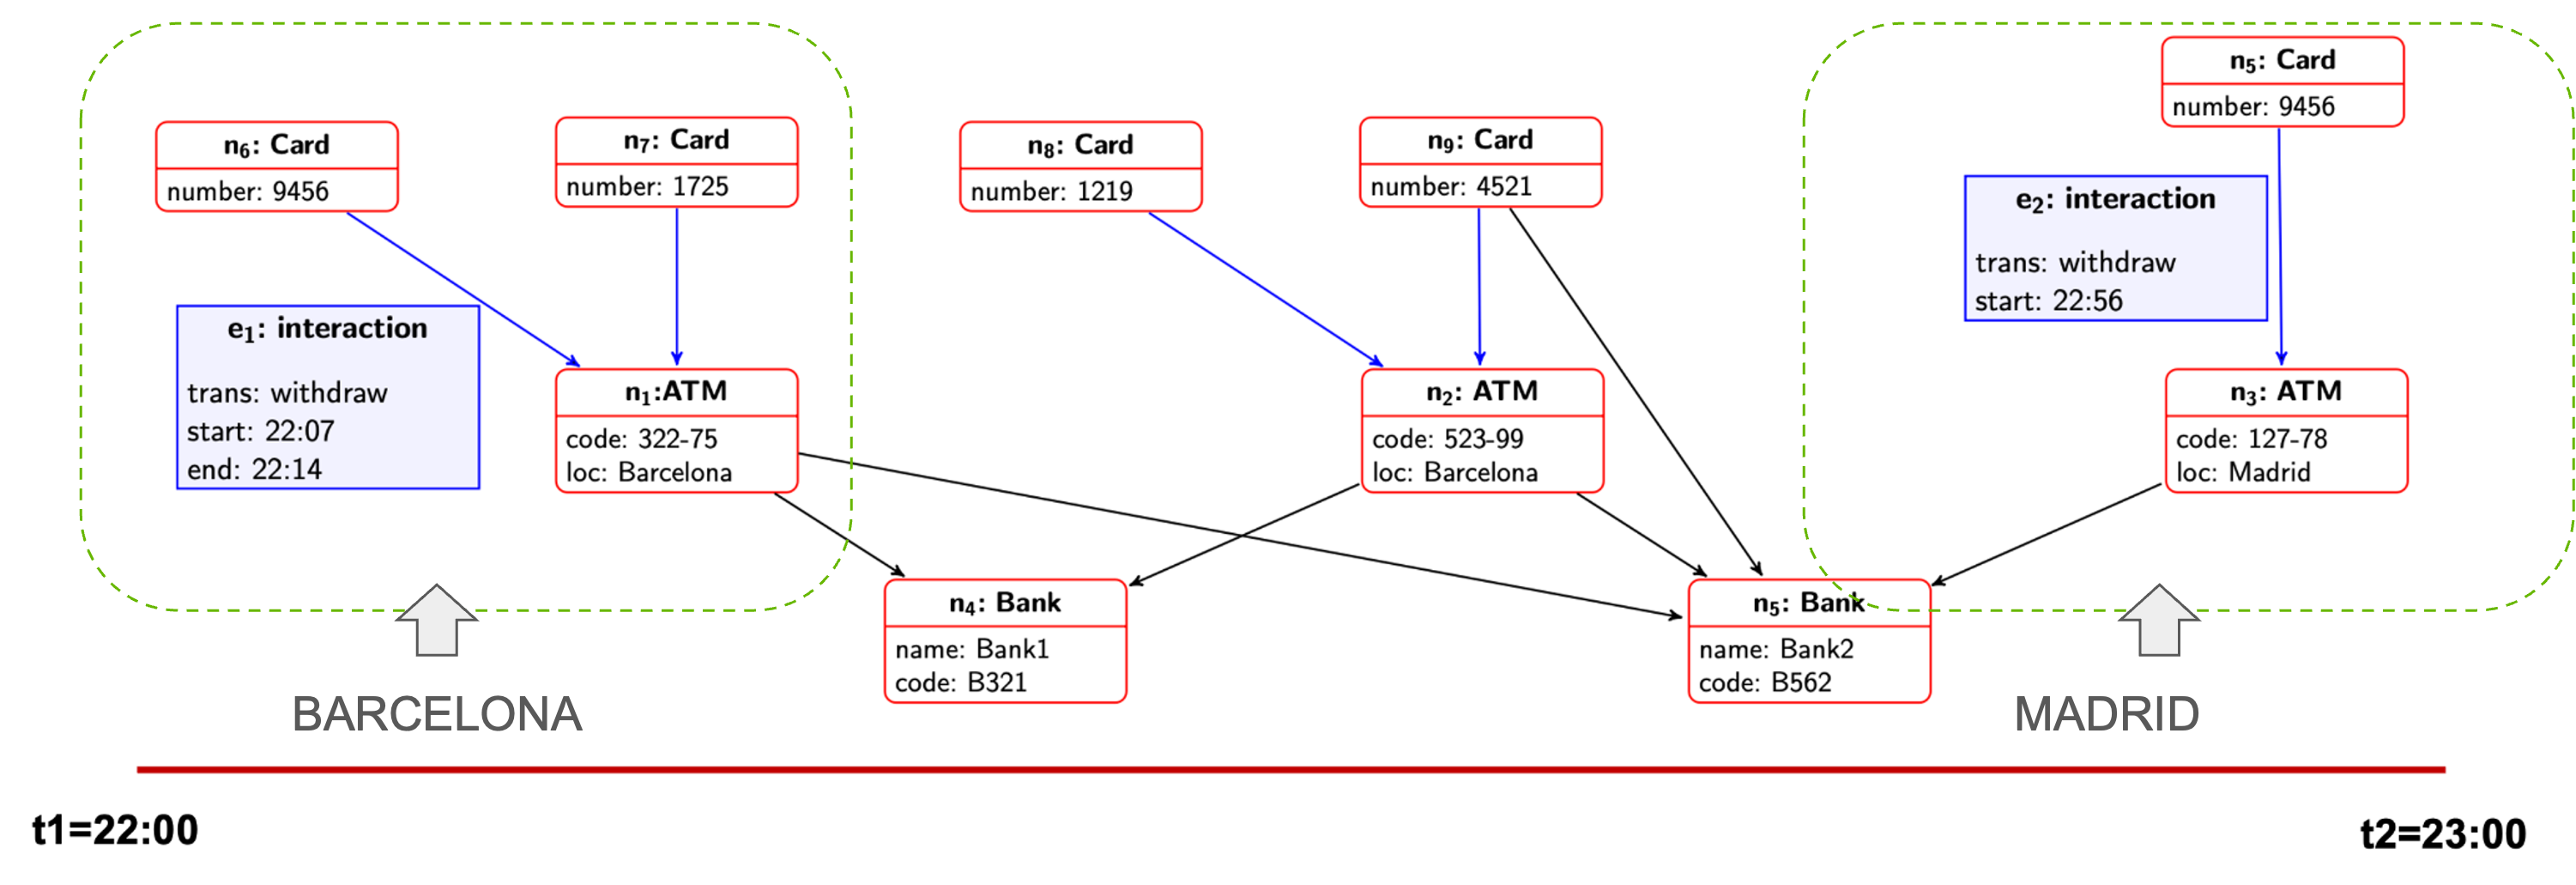
\includegraphics[width=0.8\textwidth]{images/theProblem.png}
         \caption{Example of the occurrence of anomalous ATM transactions in (a part of) a continuously evolving PG over a time interval: the card \textsf{9456} is used twice at ATMs in different cities, within one hour. However, to get from one of the cities to the other and vice versa requires more than one hour using any means of transport. This example could represent a possible case of \emph{skimming} and \emph{cloning}.}
         \label{fig:theProblem}
\end{figure}
%

\paragraph{Contribution.} The main contribution of this work is to provide, using a stream processing approach, a general technique for addressing the problem of continuous query evaluation against an evolving graph database by decomposing the datagraph into volatile and stable well defined subgraphs. Among the advantages of using the dynamic pipeline computational model are its parallel/concurrent nature and its suitability for developing real-time systems that emit results as they are computed, in a progressive way. In regards to detecting abnormal or suspicious ATM transaction, to our knowledge, most of the work addressing this topic provide a delayed detection based on predictions given by ML systems. Also, it is frequent the classical treatment of the problem by consulting log files because of the complaint of customers when detecting by themselves some weird  movement in their accounts. This involves annoying processes for customers in order to have their money back. The idea is that, in presence of some weird  finding in an ATM transaction, banks have a tool able to either ask card holders for authorizations or to take any other fraud preventing action at real-time.